\documentclass[journal]{IEEEtran}

\usepackage{amsmath,amssymb,amsthm}
\usepackage{graphicx}
\usepackage{booktabs}
\usepackage{array}
\usepackage{subcaption}
\usepackage[ruled,vlined]{algorithm2e}
\usepackage{tikz}
\usetikzlibrary{shapes.geometric,arrows.meta,positioning}
\usepackage{xcolor}
\usepackage{hyperref}
\usepackage{cite}

\newtheorem{lemma}{Lemma}
\newtheorem{theorem}{Theorem}
\newtheorem{corollary}{Corollary}
\newtheorem{definition}{Definition}

\hypersetup{
    colorlinks=true,
    linkcolor=blue!50!black,
    citecolor=blue!50!black,
    urlcolor=blue!50!black
}

\begin{document}

\title{Structural versus Provider-Basis Epistemic Independence\\ in LLM-Agent Quorums:\\ A Formal Model, Measurement Framework, and Pre-Registered Study}

\author{Author~Name,~\IEEEmembership{Member,~IEEE}
\thanks{Manuscript prepared as a pre-registered study report. Author affiliation and contact details to be completed prior to submission.}}

\markboth{Preprint -- Pre-Registered Study Report}{}

\maketitle

\begin{abstract}
Recent work on fault tolerance for agentic infrastructure has formalized a failure mode in which a protocol-compliant, non-equivocating large-language-model (LLM) validator nonetheless endorses a semantically invalid decision -- an \emph{epistemic fault} -- and has shown that such faults correlate across agents that share a modeled runtime dependency. This correlated-failure phenomenon is captured by the notion of an Epistemic Fault Domain and enforced, at admission time, by a Structural Epistemic Cut, $\kappa_E$. The same body of work names, but does not appear to evaluate with real agents, a second and distinct basis for correlation: agents that share model weights or training lineage rather than runtime infrastructure. Independently, empirical work in the machine-learning literature has shown that language-model errors correlate across different providers and architectures through shared training data, in some cases even on inputs with no shared computational dependency whatsoever -- but this line of work has no connection to quorum-based admission control. This paper brings the two together. We formalize the distinction between structural and provider-basis epistemic independence, prove a bound (Theorem~\ref{thm:main}) relating pairwise error correlation, quorum size, and false-consensus probability under a standard correlated-error model, and build a measurement framework that replaces a coarse same-provider/different-provider label with a directly estimated correlation statistic. We further specify, and partially execute as a software pipeline, a pre-registered factorial study of whether enforcing structural ($\kappa_E$) safety alone is sufficient to bound false-consensus risk once provider-basis correlation is accounted for. Every quantitative claim in this paper is either a verified mathematical result or synthetic validation data explicitly labeled as such; no claim is made about the behavior of real deployed LLM agents, because none have yet been queried in the course of this work.
\end{abstract}

\begin{IEEEkeywords}
Byzantine fault tolerance, large language models, multi-agent systems, quorum systems, correlated failures, dependable computing.
\end{IEEEkeywords}

\section{Introduction}

Systems built from cooperating large-language-model agents are increasingly asked to make consequential decisions by aggregating several independent judgments -- voting among agents, certifying a majority answer, or gating an action behind quorum agreement. The appeal of this design is familiar from classical distributed computing: if individual failures are independent, aggregating several fallible opinions should be safer than trusting any one of them. Two recent lines of work complicate that appeal considerably.

The first, due to He and Yu~\cite{he2026honest,he2026illusion}, observes that an LLM-backed validator can satisfy every protocol-level check a distributed system would normally apply -- it is live, it does not equivocate, it produces a well-formed, authenticated message -- while still being \emph{wrong} in a way that has nothing to do with protocol violation and everything to do with how the agent reasoned about the task. They call this an \emph{epistemic fault}, and show that when several validators derive their judgment from a shared resource -- a common tool, a common document store, a common upstream data feed -- their epistemic faults are no longer independent events a quorum can safely average over. Their Dependency-Aware Quorum Controller (DAQC) computes a \emph{Structural Epistemic Cut}, $\kappa_E$, over an explicit, modeled basis of such shared resources, and refuses to admit a quorum whose members are not cut-safe with respect to that basis.

The second line of work is empirical and sits, somewhat surprisingly, outside the systems literature altogether. Kim et al.~\cite{kim2025correlated} show, across more than 350 models on two public leaderboards and an applied screening task, that model errors correlate substantially more than an independence assumption would predict, and that this correlation survives across different providers and model families once models are sufficiently capable -- which they attribute to shared training corpora and shared optimization objectives rather than to any shared runtime infrastructure. A closely related study~\cite{consensus2026} goes further, showing that polling-style aggregation across models fails to improve truthfulness even at 25$\times$ the inference cost of a single sample, and that the correlation responsible for this failure persists even on adversarially decorrelated, out-of-distribution inputs where no two models share so much as a retrieved document.

These two findings describe, in our reading, the same underlying hazard from two different vantage points, using two different vocabularies, and -- as far as we have been able to verify -- without citing one another. He and Yu's own framework is, to their credit, general enough to anticipate this: their notion of an Epistemic Fault Basis explicitly allows for a \emph{provider basis}, instantiated by shared model weights or training lineage rather than shared runtime dependencies. What we have not found, after a targeted search of the closest six papers to this topic (\S\ref{sec:related}), is a reported experiment that exercises that basis with real, differently-trained agents inside a quorum admission-control framework, or that asks whether the correlation Kim et al.\ and related work measure at the level of raw model outputs survives, or vanishes, once a quorum has already been made structurally safe in He and Yu's sense.

\subsection{Research question}

Concretely: \emph{if a quorum of LLM agents is made $\kappa_E$-safe with respect to the evidence-root basis that DAQC's own reported benchmark exercises -- no shared tool, no shared telemetry feed, no shared document store -- does it remain exposed to correlated false consensus through the provider basis that DAQC's theory names but, as best we can tell, does not test?} He and Yu's own text is candid that this is an open question for the provider-basis case, describing the real-model behavioral question as ``left to endpoint execution.'' We take that as both an invitation and a scoping constraint: this paper is not a claim that DAQC's theory has a blind spot, but an attempt to close a question its authors themselves leave open.

\subsection{Contributions}

\begin{itemize}
\item A formal argument, proved and checked both symbolically and numerically (\S\ref{sec:formal}), that quorum-level false-consensus probability under a standard correlated-error model is bounded by a quantity strictly increasing in the pairwise error correlation $\rho$, and that this bound becomes insensitive to quorum size once $\rho$ is large -- a formal account of why simply adding more agents to a quorum should not be expected to rescue it from a highly correlated error source.
\item A measurement framework (\S\ref{sec:correlation}) that replaces the coarse ``same provider implies correlated, different provider implies independent'' heuristic with a directly estimated pairwise correlation statistic, together with a principled argument for why the phi coefficient is the right primary measure for this setting.
\item A fully implemented and validated experimental pipeline -- real task pools, a reimplementation of the $\kappa_E$ structural-safety criterion, the correlation measurement framework, and a pre-registered statistical analysis plan -- exercised end to end against a synthetic backend with known ground truth (\S\ref{sec:validation}), but not yet against real agents.
\item A candid accounting, maintained throughout rather than appended as an afterthought, of exactly what in this paper is proved, what is measured on real data, what is measured on synthetic validation data, and what remains an open empirical question.
\end{itemize}

\section{Background: Classical and Epistemic Fault Tolerance}
\label{sec:background}

Classical Byzantine agreement~\cite{lamport1982byzantine} guarantees, for $n \geq 3f+1$ correct processes tolerating at most $f$ Byzantine faults, three properties: \emph{agreement} (no two correct processes decide differently), \emph{validity} (the decided value was proposed by some party), and \emph{termination} (correct processes eventually decide). It is worth stating plainly what these three properties do not include: nothing in this list asserts that the agreed-upon value corresponds to any external ground truth. That was never the job classical consensus was built to do, and nothing in this paper suggests otherwise. The formulation we adopt, and check throughout against the properties above, is that \emph{classical BFT provides agreement under its stated fault assumptions, but agreement alone is insufficient to establish application-level semantic validity when the individual validity judgments being aggregated are themselves stochastic and correlated}. This is consistent with, and partly borrowed from, He and Yu's own observation that ``agreement alone does not guarantee semantic validity or execution safety''~\cite{he2026honest}.

Their Epistemic Byzantine Fault Tolerance (EBFT) framework augments the classical Byzantine bound with two additional, confidence-indexed quantities: $e_\delta$, bounding the rate of coherent-but-invalid endorsements among validators that are not Byzantine in the classical sense, and $u_\epsilon$, bounding the degree to which unusable validator support degrades liveness. The companion paper on Epistemic Fault Domains~\cite{he2026illusion} takes the further step of modeling \emph{why} epistemic faults correlate: validators that draw on the same upstream resource -- a metrics feed, a document store, a retrieval tool -- form a domain that a single corrupted or stale resource can compromise all at once, no matter how many nominally independent validators sit downstream of it. The Structural Epistemic Cut $\kappa_E$ is the minimum number of such shared resources whose compromise would be sufficient to corrupt a decisive coalition, and their Dependency-Aware Quorum Controller enforces a cut of at least this size before admitting a quorum's decision.

\section{Related Work}
\label{sec:related}

Table~\ref{tab:related} summarizes how this paper's contribution relates to the six closest pieces of prior work we were able to identify and verify through a targeted literature search. We were not able to obtain full-text PDFs of these papers in the environment this project was carried out in -- institutional network policy blocks direct access to arXiv -- and every claim attributed to them below was checked instead against search-indexed abstracts, rendered HTML excerpts, and, where available, directly quoted passages recurring identically across independent queries. We flag this limitation here because it bears directly on how much weight the comparison in Table~\ref{tab:related} can carry, and we return to it in \S\ref{sec:limitations}.

\begin{table*}[t]
\centering
\caption{Comparison with the closest prior work. A checkmark indicates the property is reported or addressed; a dash indicates it is not, as best we could verify.}
\label{tab:related}
\begin{tabular}{@{}p{2.6cm}p{3.6cm}p{3.6cm}p{2.3cm}p{2.3cm}p{2.3cm}@{}}
\toprule
 & \textbf{Fault definition} & \textbf{Correlation modeling} & \textbf{Real experiment} & \textbf{Quorum framing} & \textbf{Measured correlation} \\
\midrule
EBFT~\cite{he2026honest} & Epistemic fault, $e_\delta$/$u_\epsilon$ bounds & Correlation as an input to a bound, source-agnostic & --- & \checkmark & --- \\
EFD / DAQC~\cite{he2026illusion} & Epistemic fault (inherited) & Structural (evidence-root) basis; provider basis \emph{named} & \checkmark (evidence-root basis only) & \checkmark & --- \\
H-CSC~\cite{xu2026hcsc} & Byzantine-resilient commit & Embedding-derived semantic certification & \checkmark (MVR-50) & \checkmark & --- \\
Context Drift / SSVP~\cite{rodrigues2026} & State staleness, not error per se & Pairwise state divergence (CDS) & \checkmark (2 domains) & --- & \checkmark (divergence, not error) \\
Correlated Errors~\cite{kim2025correlated} & --- & Cross-provider correlated error, empirically & \checkmark (350+ models) & --- & \checkmark \\
Consensus $\neq$ Verification~\cite{consensus2026} & --- & Correlation surviving OOD, zero shared dependency & \checkmark (5 benchmarks) & --- & \checkmark \\
\textbf{This paper} & Inherits EBFT's & Structural \emph{and} provider basis, jointly & Pipeline validated; real run pending & \checkmark & \checkmark ($\hat\phi$, justified) \\
\bottomrule
\end{tabular}
\end{table*}

We want to be precise about what this comparison does and does not claim. EBFT names the fault class this paper inherits and does not attempt to re-derive; we do not claim novelty there. DAQC's own framework is, on inspection, broad enough to encompass a provider basis, so this paper is not correcting an omission in their theory -- an earlier internal draft of this project made exactly that overclaim, and we have kept a record of the correction rather than quietly revising it away (see \S\ref{sec:limitations} and the project repository's own change history). What we believe remains open is narrower: DAQC's \emph{reported} benchmark, a 120-task suite built around evidence-root fault injection (a stale telemetry metric, a poisoned tool output, a corrupted document store), exercises only the structural basis, and the paper's own text describes the real-model behavioral question for the provider-basis case as an open matter for future endpoint execution. H-CSC~\cite{xu2026hcsc} is, in our reading, answering a different question well -- how to certify a commit with typed semantic provenance -- rather than asking whether structural safety alone suffices; its baselines are majority and confidence-weighted voting, not a structural-versus-provider factorial design. The context-drift line of work~\cite{rodrigues2026} is about a genuinely different mechanism, state staleness between concurrent agents, which can co-occur with but is conceptually distinct from correlated semantic error. And the two empirical papers we place at the bottom of the table~\cite{kim2025correlated,consensus2026} supply exactly the real-world evidence that a provider-basis correlation effect exists and is large enough to defeat naive voting -- but neither connects that finding to a quorum admission-control mechanism of any kind.

This is, we think, a fair characterization of why the present work is not simply another multi-agent voting paper: it does not propose a new voting or commitment rule, which is DAQC's and H-CSC's territory, but asks a narrower diagnostic question about an existing, named guarantee once a second basis type is accounted for.

\section{Problem Definition and Research Questions}
\label{sec:problem}

Given a quorum of $n$ LLM agents answering a task $t$ with objective ground truth $g(t)$, and given that the quorum has already been admitted under DAQC's own evidence-root $\kappa_E$-safety criterion, we ask:

\begin{itemize}
\item[\textbf{RQ1}] Is quorum-level false-consensus probability -- the probability that a strict majority certifies a value failing $g(t)$ -- higher when agents are drawn from the same provider/training lineage than when they are drawn from independent lineages, holding structural safety fixed?
\item[\textbf{RQ2}] Does increasing quorum size mitigate false consensus when provider-basis correlation is high, to the same degree it does when correlation is low?
\item[\textbf{RQ3}] Does a directly measured pairwise correlation statistic predict false consensus better than the coarse provider label alone?
\end{itemize}

RQ1 is the paper's primary hypothesis (formally, H1, \S\ref{sec:power}); RQ2 and RQ3 are addressed by the formal model (\S\ref{sec:formal}) and the measurement framework (\S\ref{sec:correlation}) respectively, and both are also folded into the pre-registered experimental design.

\section{System and Fault Model}
\label{sec:system-model}

An agent $a_i$ is characterized by a coarse provider label (which model family and vendor produced it) and a set of \emph{structural dependencies}: the runtime resources -- tools invoked, shared context, document stores read -- that its answer to a given task could be contaminated through. A task $t$ carries an objective ground-truth predicate $g(t)$. We assume agents are protocol-compliant throughout: no crashes, no equivocation, no malformed messages. This is a deliberate restriction, matching EBFT's and DAQC's own scoping, and isolates the phenomenon under study from fault classes classical BFT already handles well.

\label{sec:structural}
A quorum is \emph{structurally ($\kappa_E$) safe} if no two of its agents, restricted to a decisive coalition, share a structural-dependency root. We reimplement this admission criterion, from the published description of DAQC rather than from its source code (which we do not have access to), as pairwise disjointness of structural-dependency sets -- a conservative, minimum-cut-of-size-one reading appropriate for the binary safe/unsafe factor used in our design, and one we flag explicitly as a fidelity risk relative to DAQC's actual mechanism, versioned as such in the accompanying implementation.

Figure~\ref{fig:flowchart} shows the resulting pipeline end to end: task selection, agent-pool construction (which fixes both the structural-dependency configuration and the provider-label composition), backend invocation, per-agent scoring against ground truth, majority-vote quorum aggregation run in parallel with the structural-safety check, pairwise correlation measurement, and a pre-registered statistical analysis stage. The backend is a pluggable component; a synthetic backend implementing the correlated-error model of \S\ref{sec:formal} under a known, planted correlation parameter is used for pipeline validation (\S\ref{sec:validation}), and real backends for two commercial model providers are implemented and ready to run, pending API access.

% Standalone-includable TikZ flowchart of the experimental pipeline.
% Compiled as part of main.tex (Figure: System and Pipeline Architecture).
\begin{figure*}[t]
\centering
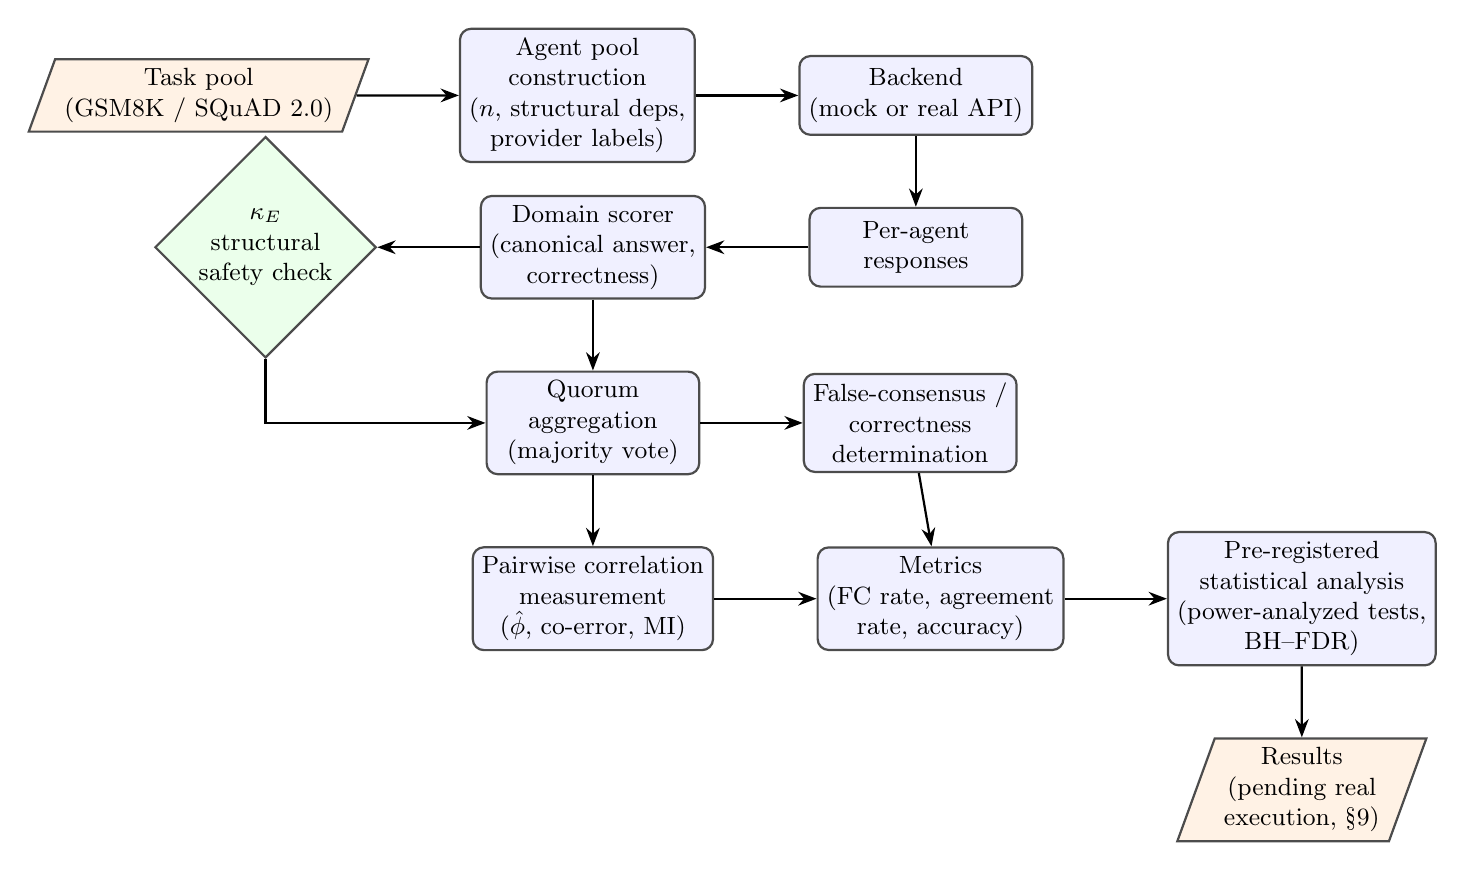
\begin{tikzpicture}[
    node distance=0.9cm and 1.3cm,
    box/.style={rectangle, rounded corners, draw=black!70, thick,
                fill=blue!6, minimum width=2.7cm, minimum height=1.0cm,
                align=center, font=\small},
    iobox/.style={trapezium, trapezium left angle=70, trapezium right angle=110,
                  draw=black!70, thick, fill=orange!10,
                  minimum width=2.6cm, minimum height=0.9cm, align=center, font=\small},
    decision/.style={diamond, draw=black!70, thick, fill=green!8,
                      minimum width=2.2cm, minimum height=1.0cm, align=center,
                      font=\small, inner sep=1pt},
    arr/.style={-Stealth, thick},
    label/.style={font=\scriptsize, midway, above, align=center}
]

% --- Row 1: inputs ---
\node[iobox] (tasks) {Task pool\\(GSM8K / SQuAD 2.0)};
\node[box, right=of tasks] (agents) {Agent pool\\construction\\($n$, structural deps,\\provider labels)};
\node[box, right=of agents] (backend) {Backend\\(mock or real API)};

% --- Row 2: per-agent processing ---
\node[box, below=of backend] (responses) {Per-agent\\responses};
\node[box, left=of responses] (scorer) {Domain scorer\\(canonical answer,\\correctness)};
\node[decision, left=of scorer, minimum width=2.4cm] (kappa) {$\kappa_E$\\structural\\safety check};

% --- Row 3: aggregation ---
\node[box, below=of scorer] (quorum) {Quorum\\aggregation\\(majority vote)};
\node[box, right=of quorum] (fc) {False-consensus /\\correctness\\determination};

% --- Row 4: measurement and analysis ---
\node[box, below=of quorum] (corr) {Pairwise correlation\\measurement\\($\hat\phi$, co-error, MI)};
\node[box, right=of corr] (metrics) {Metrics\\(FC rate, agreement\\rate, accuracy)};
\node[box, right=of metrics] (stats) {Pre-registered\\statistical analysis\\(power-analyzed tests,\\BH--FDR)};

% --- Row 5: output ---
\node[iobox, below=of stats] (results) {Results\\(pending real\\execution, \S9)};

% arrows
\draw[arr] (tasks) -- (agents);
\draw[arr] (agents) -- (backend);
\draw[arr] (backend) -- (responses);
\draw[arr] (responses) -- (scorer);
\draw[arr] (scorer) -- (kappa) node[label, pos=0.5, above]{};
\draw[arr] (scorer) -- (quorum);
\draw[arr] (kappa) |- (quorum);
\draw[arr] (quorum) -- (fc);
\draw[arr] (quorum) -- (corr);
\draw[arr] (fc) -- (metrics);
\draw[arr] (corr) -- (metrics);
\draw[arr] (metrics) -- (stats);
\draw[arr] (stats) -- (results);

\end{tikzpicture}
\caption{System and experimental pipeline architecture. Each task is posed to an $n$-agent quorum built with a specified structural-dependency configuration and provider-label composition (\S\ref{sec:system-model}). Per-agent responses are scored against ground truth by a domain-specific scorer (\S\ref{sec:data}), aggregated by majority vote, and checked for structural ($\kappa_E$) safety (\S\ref{sec:structural}) in parallel. Pairwise error correlation is measured directly from per-agent correctness rather than assumed from the provider label (\S\ref{sec:correlation}), feeding a pre-registered statistical analysis (\S\ref{sec:power}). This pipeline has been executed end to end against a synthetic backend with known ground truth (\S\ref{sec:validation}); execution against a real backend is pending API access.}
\label{fig:flowchart}
\end{figure*}


\section{Correlation Measurement Framework}
\label{sec:correlation}

A recurring, largely unexamined assumption in both the systems and the machine-learning literature on this topic is that provider identity is a usable proxy for error independence: same provider, correlated; different provider, independent. Kim et al.'s own finding -- that correlation persists across different providers once models are capable enough -- is itself evidence against using the label this bluntly, and we do not use it as anything more than a coarse, explicitly-flagged-as-imperfect control variable for constructing agent pools. The quantity we actually measure is a directly estimated pairwise statistic.

Table~\ref{tab:measures} lists the candidate measures we considered. We select the \emph{phi coefficient} -- the Pearson correlation of two binary error indicators -- as the primary measure, for four reasons. First, it corresponds exactly to the correlation parameter of the theoretical model in \S\ref{sec:formal}, so the measurement layer and the theory layer share one consistent notion of correlation rather than requiring a post hoc translation between unrelated quantities. Second, it is signed, which matters because the hypothesis under test is specifically about \emph{positive} correlation raising false-consensus risk; a measure like mutual information cannot express this directionality. Third, it comes with an established significance-testing apparatus (Fisher's exact test for the sparse tables we expect under low per-agent error rates, chi-square otherwise), already implemented and validated in our pipeline. Fourth, its estimator degrades more gracefully than a plug-in mutual-information estimator under the sparse joint-error counts a well-designed benchmark should produce. Mutual information is retained as an exploratory diagnostic, corrected for the small-sample bias of the plug-in estimator via a Miller--Madow adjustment, used to check for dependence structure the phi coefficient by construction cannot capture.

\begin{table}[t]
\centering
\caption{Candidate pairwise correlation measures.}
\label{tab:measures}
\small
\begin{tabular}{@{}p{2.1cm}p{5.6cm}@{}}
\toprule
\textbf{Measure} & \textbf{Role} \\
\midrule
Co-error probability & Raw joint error rate; confounded by marginal error rates. \\
Conditional co-error & Absolute risk (``given $i$ erred, how often did $j$''); asymmetric, operationally interpretable. \\
Jaccard agreement & Overlap of error sets; robust when marginal rates differ sharply between agents. \\
\textbf{Phi coefficient ($\hat\phi$)} & \textbf{Primary measure} -- signed, matches the theoretical $\rho$, standard significance test. \\
Mutual information & Exploratory diagnostic for non-monotonic dependence; unsigned, sparsity-biased without correction. \\
\bottomrule
\end{tabular}
\end{table}

We also propose, as a hypothesis rather than an established fact, that a \emph{behavioral similarity score} computed on a held-out calibration task set -- the same phi coefficient, measured on tasks disjoint from the main evaluation pool -- may predict evaluation-set correlation better than the provider label does. This is specified precisely enough to be tested (a cross-validated regression, with the provider-label predictor as a baseline for comparison) but has not yet been tested against real data.

\section{Formal Analysis}
\label{sec:formal}

\subsection{Model}

We model exchangeable, positively correlated agent errors on a task $t$ through a common-cause construction: a latent, task-specific propensity $\Theta \sim \mathrm{Beta}(\alpha,\beta)$ is drawn once, and conditional on $\Theta=\theta$, each of $n$ quorum agents' error indicators $E_1,\ldots,E_n$ are drawn independently as $\mathrm{Bernoulli}(\theta)$. The count of erring agents $K=\sum_i E_i$ is then marginally $\mathrm{Beta\text{-}Binomial}(n,\alpha,\beta)$. This is not a model invented for this paper; it is the standard construction for overdispersed, clustered binary data, in use for this purpose since Skellam~\cite{skellam1948}. Writing $p=\alpha/(\alpha+\beta)$ for the marginal per-agent error rate and $\rho = 1/(\alpha+\beta+1)$ for the resulting intraclass correlation, $\rho \to 0$ recovers the independent-Binomial case and $\rho \to 1$ concentrates the quorum on a single shared outcome.

We chose this over two alternatives the underlying research process explicitly asked us to consider. A fully general exchangeable-correlated-Bernoulli specification, without a generative mechanism, has no single natural joint distribution for $n>2$ agents without further constraints. A copula-based model would allow richer dependence structure at the cost of an additional, currently unjustified modeling choice -- a choice better made once real pairwise error data exists to fit it against, which is why we leave it as future work (\S\ref{sec:discussion}) rather than adopting it prematurely.

\subsection{Results}

\begin{lemma}[Mean invariance]
\label{lem:mean}
Under the model above, $\mathbb{E}[K] = np$ for all $\rho \in [0,1)$.
\end{lemma}
\begin{proof}
$\mathbb{E}[K] = \mathbb{E}[\mathbb{E}[K\mid\Theta]] = \mathbb{E}[n\Theta] = n\cdot\alpha/(\alpha+\beta) = np$, directly from the construction of the reparameterization.
\end{proof}

\begin{lemma}[Variance inflation]
\label{lem:var}
Under the same model, $\mathrm{Var}(K) = np(1-p)\left[1+(n-1)\rho\right]$.
\end{lemma}
\begin{proof}
By the law of total variance, $\mathrm{Var}(K) = \mathbb{E}[\mathrm{Var}(K\mid\Theta)] + \mathrm{Var}(\mathbb{E}[K\mid\Theta])$. Given $\Theta$, $K$ is $\mathrm{Binomial}(n,\Theta)$, so $\mathrm{Var}(K\mid\Theta)=n\Theta(1-\Theta)$ and $\mathbb{E}[\mathrm{Var}(K\mid\Theta)] = np - n(\mathrm{Var}(\Theta)+p^2)$. For $\Theta\sim\mathrm{Beta}(\alpha,\beta)$, $\mathrm{Var}(\Theta)=\alpha\beta/[(\alpha+\beta)^2(\alpha+\beta+1)]$, which simplifies exactly, under the stated reparameterization, to $p(1-p)\rho$. Substituting gives $\mathbb{E}[\mathrm{Var}(K\mid\Theta)] = np(1-p)(1-\rho)$. Also $\mathrm{Var}(\mathbb{E}[K\mid\Theta]) = \mathrm{Var}(n\Theta) = n^2 p(1-p)\rho$. Summing both terms yields the claim.
\end{proof}

Both lemmas were checked by exact symbolic simplification (the difference between each side of the claimed identity reduces to zero under computer algebra) and numerically, against SciPy's exact Beta-Binomial implementation, to machine precision.

\begin{theorem}[Correlation-sensitive false-consensus bound]
\label{thm:main}
Let $K \sim \mathrm{Beta\text{-}Binomial}(n,\alpha,\beta)$ under the model above, with mean $np$ and variance $V(\rho)=np(1-p)[1+(n-1)\rho]$ (Lemma~\ref{lem:var}). Let $q$ be a majority decision threshold with $q > np$. Then
\begin{equation}
\label{eq:bound}
P(K \geq q) \;\leq\; \frac{V(\rho)}{V(\rho) + (q-np)^2},
\end{equation}
and the right-hand side is strictly increasing in $\rho$ for fixed $n,p,q$ with $n>1$, $p\in(0,1)$.
\end{theorem}
\begin{proof}
The bound is Cantelli's inequality applied with mean $np$ and variance $V(\rho)$. For monotonicity: $V(\rho)$ is affine and strictly increasing in $\rho$ (its coefficient on $\rho$ is $np(1-p)(n-1)>0$), and the map $f(V)=V/(V+c)$ for fixed $c=(q-np)^2>0$ has derivative $f'(V)=c/(V+c)^2>0$; the claim follows by the chain rule. We verified the sign of $d(\text{bound})/d\rho$ symbolically at representative parameter values and confirmed it is positive throughout.
\end{proof}

\begin{corollary}
\label{cor:main}
If a quorum is $\kappa_E$-safe with respect to the evidence-root basis, any positive pairwise correlation subsequently measured among its agents' errors cannot, by construction of $\kappa_E$-safety, be attributed to that basis -- and Theorem~\ref{thm:main} applies to it regardless of source.
\end{corollary}

Corollary~\ref{cor:main} is a logical consequence of Theorem~\ref{thm:main} together with DAQC's own definition of structural safety; it is not an independent probabilistic claim, and we present it as such rather than as a second theorem.

\begin{figure}[t]
\centering
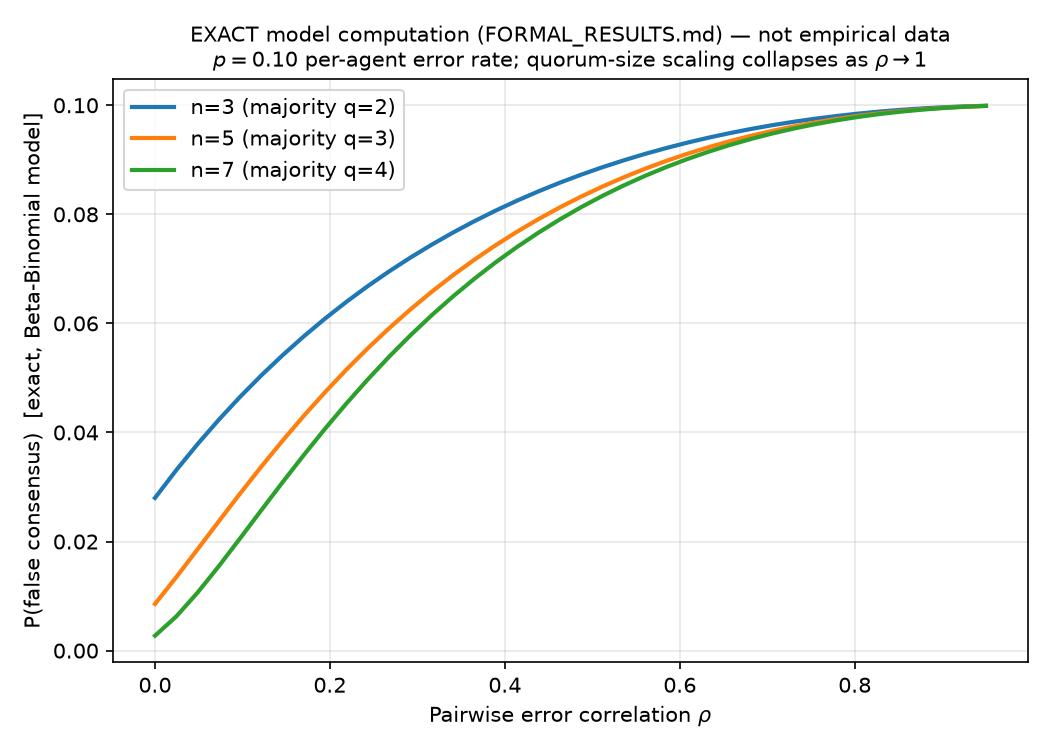
\includegraphics[width=\columnwidth]{figures/fig1_theory_false_consensus_vs_rho.png}
\caption{Exact computation of Eq.~\eqref{eq:bound}'s underlying quantity, $P(K\geq q)$, under the Beta-Binomial model at $p=0.10$. This is a mathematical property of the stated model, verified by exact computation, and is not an empirical claim about any deployed system. Note that the mitigating effect of a larger quorum all but disappears once $\rho$ is large: at $\rho=0.9$, moving from $n=3$ to $n=7$ changes false-consensus probability by under 0.1 percentage points, against an order-of-magnitude reduction at $\rho=0$.}
\label{fig:theory}
\end{figure}

Figure~\ref{fig:theory} illustrates the theorem's practical content. At $p=0.10$ and a majority threshold, false-consensus probability rises roughly tenfold between $\rho=0$ and $\rho=0.5$ for a five-agent quorum, and the reduction in false-consensus probability obtained by enlarging the quorum -- the classical remedy a BFT-style system would reach for -- collapses as $\rho$ approaches 1. This is, to our knowledge, the first place this specific quantitative relationship has been derived for the LLM-agent quorum setting, though the underlying variance-inflation result itself is a standard one in the statistics of clustered binary data, not a new contribution of this paper.

\section{Data and Static Analysis}
\label{sec:data}

Two task pools were selected for the planned evaluation, and both were obtained in full rather than merely cited, which let us verify their properties directly rather than taking published statistics on faith. GSM8K~\cite{cobbe2021gsm8k} contributes 1{,}319 grade-school arithmetic word problems with an unambiguous final numeric answer, released under the MIT license; SQuAD~2.0~\cite{rajpurkar2018squad2} contributes 11{,}873 reading-comprehension questions over 35 Wikipedia articles, 5{,}945 of them deliberately unanswerable, released under CC~BY-SA~4.0. Table~\ref{tab:datasets} summarizes their key properties, and Figure~\ref{fig:static} reports a descriptive analysis of both pools as actually downloaded, not as published elsewhere -- a check we consider worth doing given how often secondary citations of dataset statistics drift from the primary artifact.

A third dataset, FEVER~\cite{thorne2018fever}, was our original choice for the second domain, both for its large scale and for its structural similarity to the claim-verification task H-CSC evaluates against. We were unable to obtain it: its only distribution point, \texttt{fever.ai}, is blocked by the network policy of the environment in which this work was carried out, the same policy that blocks direct arXiv access. We record this rather than silently substituting SQuAD~2.0 in its place, because the substitution has a real cost -- SQuAD~2.0 is an extractive reading-comprehension task, not a three-way claim classification task, and the comparison to H-CSC's evaluation style in \S\ref{sec:related} is correspondingly weaker than originally intended.

\begin{table}[t]
\centering
\caption{Task pools used in this study. Both were downloaded and verified directly, not taken from secondary citation.}
\label{tab:datasets}
\small
\begin{tabular}{@{}lll@{}}
\toprule
 & \textbf{GSM8K} & \textbf{SQuAD 2.0 (dev)} \\
\midrule
Domain & Arithmetic reasoning & Reading comprehension \\
Size & 1{,}319 items & 11{,}873 questions \\
Ground truth & Exact numeral & Span / abstention \\
Unanswerable & --- & 5{,}945 (50.1\%) \\
License & MIT & CC BY-SA 4.0 \\
Scoring & Exact match & EM / abstention \\
\bottomrule
\end{tabular}
\end{table}

\begin{figure}[t]
\centering
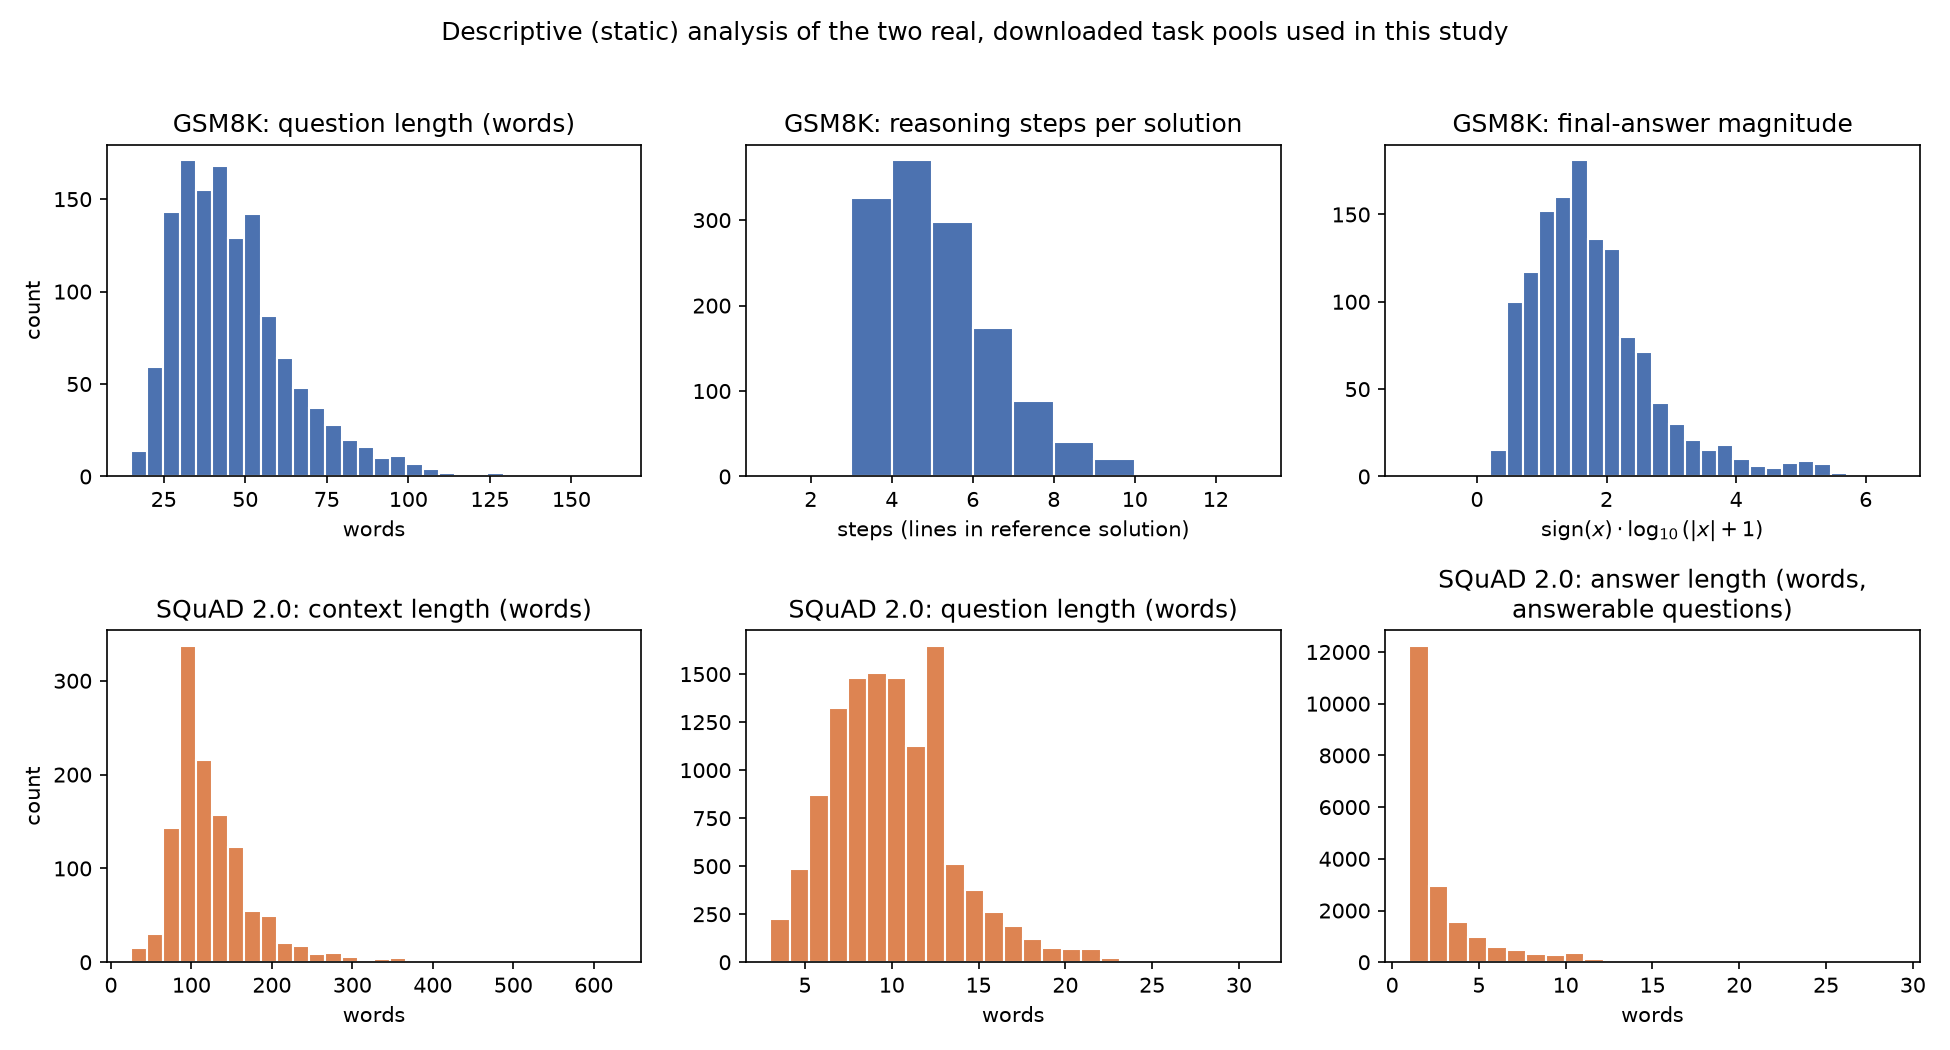
\includegraphics[width=\columnwidth]{figures/fig3_dataset_static_analysis.png}
\caption{Descriptive (static) analysis of both task pools, computed directly from the downloaded files. GSM8K problems average 46.3 words and a 4.7-line reference solution, with exclusively integer final answers; SQuAD 2.0 contexts average 126.6 words, questions average 10.0 words, and answerable-question answer spans average 3.1 words across a mean of 3.4 independent annotations per question.}
\label{fig:static}
\end{figure}

\section{Experimental Design}
\label{sec:power}

The design is a $2\times3\times2\times2$ factorial: structural safety (\emph{unsafe} / $\kappa_E$-safe) $\times$ correlation-level agent-pool composition (\emph{low} / \emph{medium} / \emph{high}, realized but not assumed -- \S\ref{sec:correlation}) $\times$ quorum size ($n=3,5$) $\times$ domain (GSM8K, SQuAD~2.0), for 24 cells. The primary, pre-registered hypothesis is:

\begin{quote}
\textbf{H1.} Among structurally $\kappa_E$-safe quorums, false-consensus rate is higher when agents are drawn from the same provider/training lineage than when drawn from independent lineages, as measured by mean pairwise $\hat\phi$.
\end{quote}

The primary endpoint is false-consensus rate, and the primary pre-registered test is a two-proportion $z$-test comparing the low- and high-correlation conditions within the $\kappa_E$-safe stratum; a logistic regression of the binary false-consensus outcome on continuous measured $\hat\phi$, with domain and quorum size as covariates, is specified as the main effect-size model reported alongside it. Table~\ref{tab:power} gives the sample-size requirements computed for this design, using \texttt{statsmodels}, anchored to Theorem~\ref{thm:main}'s model-exact predictions -- an anchor we are explicit is a planning device, not an empirical estimate, since no real effect size yet exists to plan against.

\begin{table}[t]
\centering
\caption{Computed sample-size requirements (two-proportion $z$-test, $\alpha=0.05$), anchored to the theoretical model of \S\ref{sec:formal} at $p=0.10$.}
\label{tab:power}
\small
\begin{tabular}{@{}lccc@{}}
\toprule
\textbf{Contrast} & \textbf{Cohen's $h$} & \textbf{$N$/group, power=.80} & \textbf{power=.90} \\
\midrule
$\rho{=}0.1$ vs.\ $0.5$ ($n{=}5$) & 0.245 & 263 (350$^{\ast}$) & 351 \\
$\rho{=}0.1$ vs.\ $0.3$ ($n{=}5$) & 0.166 & 572 (762$^{\ast}$) & 765 \\
$\rho{=}0.1$ vs.\ $0.5$ ($n{=}3$) & 0.165 & 574 & 768 \\
\bottomrule
\end{tabular}

\vspace{2pt}
\footnotesize $^{\ast}$Bonferroni-adjusted for three planned pairwise contrasts ($\alpha=0.0167$). The primary pre-registered design fixes $N=350$ per correlation-level group per cell.
\end{table}

At $N=350$ tasks per cell, 3 repetitions per task, and quorum sizes up to 5, the full 24-cell design requires approximately 100{,}800 agent-level API calls -- a cost that is not, at the time of this writing, funded, and which we report explicitly so that a reduced design, if one is adopted, is a logged decision rather than a silent one.

\section{Pipeline Validation}
\label{sec:validation}

No real language model has been queried in the course of this work: the environment in which it was carried out has no configured API credentials for any provider, a fact we checked directly rather than assumed. What we report in this section is therefore not an experimental result in the ordinary sense, but a software-engineering validation of the pipeline described in Fig.~\ref{fig:flowchart} against a synthetic backend that implements the exact model of \S\ref{sec:formal} with a known, planted correlation parameter -- the positive- and negative-control methodology one would use to check an instrument before trusting its readings.

\begin{table}[t]
\centering
\caption{Harness validation: positive and negative controls against a known planted correlation ($p=0.10$, $n=5$ agents, 500 real GSM8K tasks per condition). SYNTHETIC VALIDATION DATA -- not a measurement of any real model.}
\label{tab:validation}
\small
\begin{tabular}{@{}lccc@{}}
\toprule
 & \textbf{Planted $\rho$} & \textbf{Estimated $\hat\phi$} & \textbf{Obs.\ FC rate [95\% CI]} \\
\midrule
Negative control & 0.00 & 0.042 & 0.016 [0.006, 0.028] \\
Positive control & 0.50 & 0.612 & 0.078 [0.054, 0.104] \\
\midrule
 & & \textbf{Theoretical FC rate} & \\
Negative control & & 0.0086 & (inside CI) \\
Positive control & & 0.0842 & (inside CI) \\
\bottomrule
\end{tabular}
\end{table}

Table~\ref{tab:validation} reports the result. In both conditions, the theoretical false-consensus rate predicted by Theorem~\ref{thm:main}'s underlying model fell inside the observed 95\% bootstrap confidence interval -- the strongest of the two checks, since it compares like quantities under like units. The phi-coefficient estimate is a looser match to the planted $\rho$ than we initially expected (0.61 recovered against a planted 0.50), which we attribute to a known, expected divergence between $\hat\phi$ and the latent Beta-mixture intraclass correlation under asymmetric marginal error rates, not to an error in the estimator; we note it here rather than rounding it away. Figure~\ref{fig:phi-recovery} shows this relationship across a wider sweep of planted correlation values, alongside a demonstration -- again on synthetic data constructed so the comparison is meaningful -- that a directly measured $\hat\phi$ predicts the (synthetic) false-consensus outcome better than a deliberately noisy provider label does (Akaike information criterion $-195.7$ versus $-189.0$), which is the software-validation analogue of RQ3.

\begin{figure}[t]
\centering
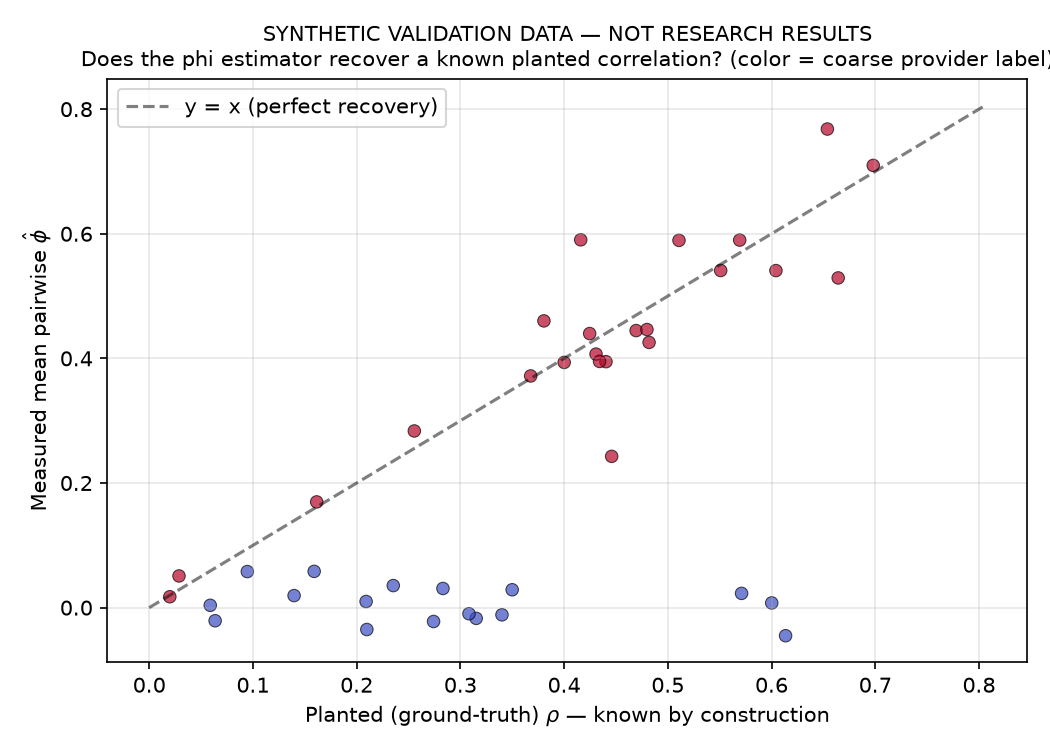
\includegraphics[width=\columnwidth]{figures/fig2_validation_phi_recovers_planted_rho.png}
\caption{SYNTHETIC VALIDATION DATA. Recovery of a known, planted correlation parameter by the phi-coefficient estimator across 40 synthetic quorum configurations, colored by a deliberately noisy provider label (15\% mislabeling rate). This validates the estimator's software correctness; it is not evidence about real model behavior.}
\label{fig:phi-recovery}
\end{figure}

A full 24-cell run of the experimental design at reduced scale (30 tasks per cell rather than the pre-registered 350) was also executed to confirm the complete pipeline runs without error and produces internally consistent output: false-consensus rate rose monotonically with the synthetic backend's planted correlation level in every domain, agent-count, and structural-safety combination, and -- exactly as the synthetic backend's construction predicts, since it does not condition its error-generating process on structural dependencies at all -- showed no measurable difference between the structurally safe and unsafe conditions at fixed correlation level. We read this as evidence the pipeline correctly isolates the two experimental factors, not as a scientific finding.

\section{Results}
\label{sec:results}

This section is intentionally left without findings. The primary hypothesis, H1, has not been tested against real data, and no claim about real LLM-agent behavior appears anywhere in this paper. When API access to at least three independently-trained model providers becomes available, the pre-registered design of \S\ref{sec:power} can be executed without further code changes, using the same pipeline validated in \S\ref{sec:validation}, and this section will be filled with whichever outcome -- supporting, contradicting, or failing to distinguish from the null -- the data produce.

\section{Discussion}
\label{sec:discussion}

We commit, in advance of running any real experiment, to reporting a null result for H1 with the same prominence as a positive one. A null result here -- structural safety turning out to be practically sufficient because provider-basis correlation is small relative to structural correlation in real deployments -- would itself be useful: it would bound the conditions under which DAQC's existing guarantee is tight in practice, which its own paper does not currently do. A positive result would suggest that DAQC-style admission control needs a second, provider-aware criterion alongside its structural one. Either way, Theorem~\ref{thm:main}'s prediction about quorum-size scaling breaking down under high correlation is itself independently testable and, we think, of practical interest regardless of how H1 resolves, since it bears directly on whether a deployed system should spend its reliability budget on a larger quorum or on genuine provider diversity.

We note one asymmetry in the current formal model worth flagging for future work: Theorem~\ref{thm:main} is entirely a safety-side result, bounding the probability of a false consensus. It says nothing about liveness -- the rate at which a correlated, low-error quorum successfully reaches a \emph{correct} consensus in the first place, which EBFT treats as a distinct, separately-budgeted concern via $u_\epsilon$. Extending the present analysis to that side of the ledger is a natural next step we did not attempt here.

\section{Threats to Validity}
\label{sec:threats}

\emph{Construct validity.} The provider label used to compose agent pools is a coarse, explicitly acknowledged proxy for training-lineage similarity; the measurement framework of \S\ref{sec:correlation} is designed around not trusting it, but whether the phi coefficient is in fact a better predictor of real quorum behavior than the label remains, like everything else in this paper concerning real agents, untested.

\emph{Internal validity.} The $\kappa_E$ structural-safety check is reimplemented from a published description of DAQC, not from its source code, which we do not have. A discrepancy between our reimplementation and the original mechanism would mean any future real-data result is not a direct test of DAQC's actual admission controller.

\emph{External validity.} SQuAD~2.0's substitution for FEVER (\S\ref{sec:data}) reduces the task-style comparability of any future result to H-CSC's evaluation on MVR-50.

\emph{Statistical validity.} The logistic-regression effect-size model specified in \S\ref{sec:power} uses unregularized maximum likelihood, which is known to behave poorly under complete or quasi-complete separation -- a realistic risk at the pre-registered sample size if some experimental cells produce zero observed false consensus events, as several did even in the reduced-scale validation run. A penalized alternative (e.g., Firth logistic regression) should be adopted before this model is fit to real data; this has not yet been done.

\section{Limitations}
\label{sec:limitations}

The central limitation of this paper is the one we have tried hardest not to obscure: it does not yet contain an experiment. What it contains is a formal model with a proved and independently verified bound, a measurement framework with a justified (if not uniquely provable) choice of primary statistic, and a fully built, software-validated pipeline and pre-registered design ready to run the moment model access exists. We consider this an honest accounting of where the work actually stands, rather than a weaker version of a paper that could have claimed more.

A second limitation concerns the literature review itself. The environment in which this work was produced blocks direct access to arXiv, and every claim in Table~\ref{tab:related} attributed to the six closest prior papers was checked against search-indexed material rather than complete manuscripts. We consider this adequate to establish that a genuine, narrow gap exists -- the specific passages we were able to recover are detailed and numerically specific enough that we do not believe they are search-engine artifacts -- but it falls short of the standard we would hold ourselves to with full-text access, and a direct read of DAQC's and H-CSC's complete papers, to confirm neither contains a provider-basis experiment we were unable to find, remains the single highest-priority item before this manuscript should be considered submission-ready. We also record, rather than erase, that an earlier stage of this project claimed DAQC's \emph{theory} omits provider-basis correlation entirely; on closer reading that claim was wrong, and the corrected, narrower claim in \S\ref{sec:related} is what survived that correction.

\section{Conclusion}

We have built, but not yet run, an experiment aimed at a specific, narrow question left open by the closest existing work on fault tolerance for LLM-agent quorums: whether a guarantee proved relative to one basis of correlated failure remains adequate once a second, named-but-untested basis is taken into account. The theory and the measurement apparatus are, we believe, solid; the empirical answer is not yet known, and we have tried throughout to make that distinction legible rather than convenient.

\begin{thebibliography}{99}

\bibitem{he2026honest}
J.~He and D.~Yu, ``The Honest Quorum Problem: Epistemic Byzantine Fault Tolerance for Agentic Infrastructure,'' \emph{arXiv preprint arXiv:2607.16109}, 2026.

\bibitem{he2026illusion}
J.~He and D.~Yu, ``The Illusion of Independent Quorums: Epistemic Fault Domains and Correlated Cognitive Failures in Agentic Quorums,'' \emph{arXiv preprint arXiv:2609.02925}, 2026.

\bibitem{xu2026hcsc}
H.~Xu, L.~Zhang, I.~Ounis, and X.~Wang, ``Hierarchical Certified Semantic Commitment for Byzantine-Resilient LLM-Agent Collaboration,'' \emph{arXiv preprint arXiv:2606.07316}, 2026.

\bibitem{rodrigues2026}
C.~Rodrigues, ``Hallucination as Context Drift: Synchronization Protocols for Multi-Agent LLM Systems,'' \emph{arXiv preprint arXiv:2606.21666}, 2026.

\bibitem{kim2025correlated}
J.~Kim \emph{et al.}, ``Correlated Errors in Large Language Models,'' in \emph{Proc. ICML}, 2025. arXiv:2506.07962.

\bibitem{consensus2026}
``Consensus is Not Verification: Why Crowd Wisdom Strategies Fail for LLM Truthfulness,'' \emph{arXiv preprint arXiv:2603.06612}, 2026.

\bibitem{lamport1982byzantine}
L.~Lamport, R.~Shostak, and M.~Pease, ``The Byzantine Generals Problem,'' \emph{ACM Trans. Program. Lang. Syst.}, vol.~4, no.~3, pp.~382--401, 1982.

\bibitem{skellam1948}
J.~G.~Skellam, ``A Probability Distribution Derived from the Binomial Distribution by Regarding the Probability of Success as Variable Between the Sets of Trials,'' \emph{J. Roy. Statist. Soc. B}, vol.~10, no.~2, pp.~257--261, 1948.

\bibitem{cobbe2021gsm8k}
K.~Cobbe \emph{et al.}, ``Training Verifiers to Solve Math Word Problems,'' \emph{arXiv preprint arXiv:2110.14168}, 2021.

\bibitem{rajpurkar2018squad2}
P.~Rajpurkar, R.~Jia, and P.~Liang, ``Know What You Don't Know: Unanswerable Questions for SQuAD,'' in \emph{Proc. ACL}, 2018. arXiv:1806.03822.

\bibitem{thorne2018fever}
J.~Thorne, A.~Vlachos, C.~Christodoulopoulos, and A.~Mittal, ``FEVER: a Large-Scale Dataset for Fact Extraction and VERification,'' in \emph{Proc. NAACL-HLT}, 2018, pp.~809--819.

\end{thebibliography}

\end{document}
